\documentclass[]{article}
\usepackage{graphicx}
\usepackage[left=0.40in,top=0.3in,right=0.75in,bottom=0.1in]{geometry}
%opening
\title{Problem Set 7}
\author{Rodrigo Chavez Zavaleta}

\begin{document}

\maketitle

\section{Problem 1}
We are asked to show that the xyz coordinates generated by the C standard library lie on planes. Unfortunately, I was not able to run the generator on my local machine, although I am using Ubuntu 20.04 and called the "libc.so" library.

We then plot the points imported from rand\_points.txt and plot them in 3D then move around the view. We find that setting the view to (0, 60) showcases the planes we are looking for.
\begin{figure}[h]
	\centering
	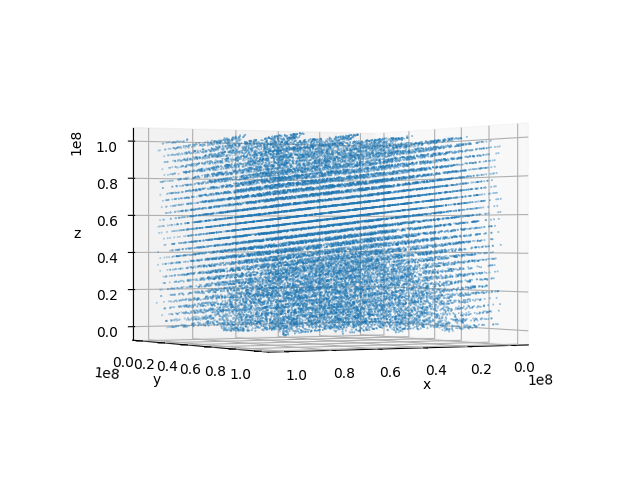
\includegraphics[width=0.8\linewidth]{Results/q1a.png}
\end{figure}

Now we are asked if we see the same using a python random number generator. We use numpy's random generator, and again plot the 3d points. we do not see the same 'planes' pattern, and we show here the points rotated by a half turn in twelve steps, which fails to find a pattern.

\begin{figure}[bp!]
	\centering
	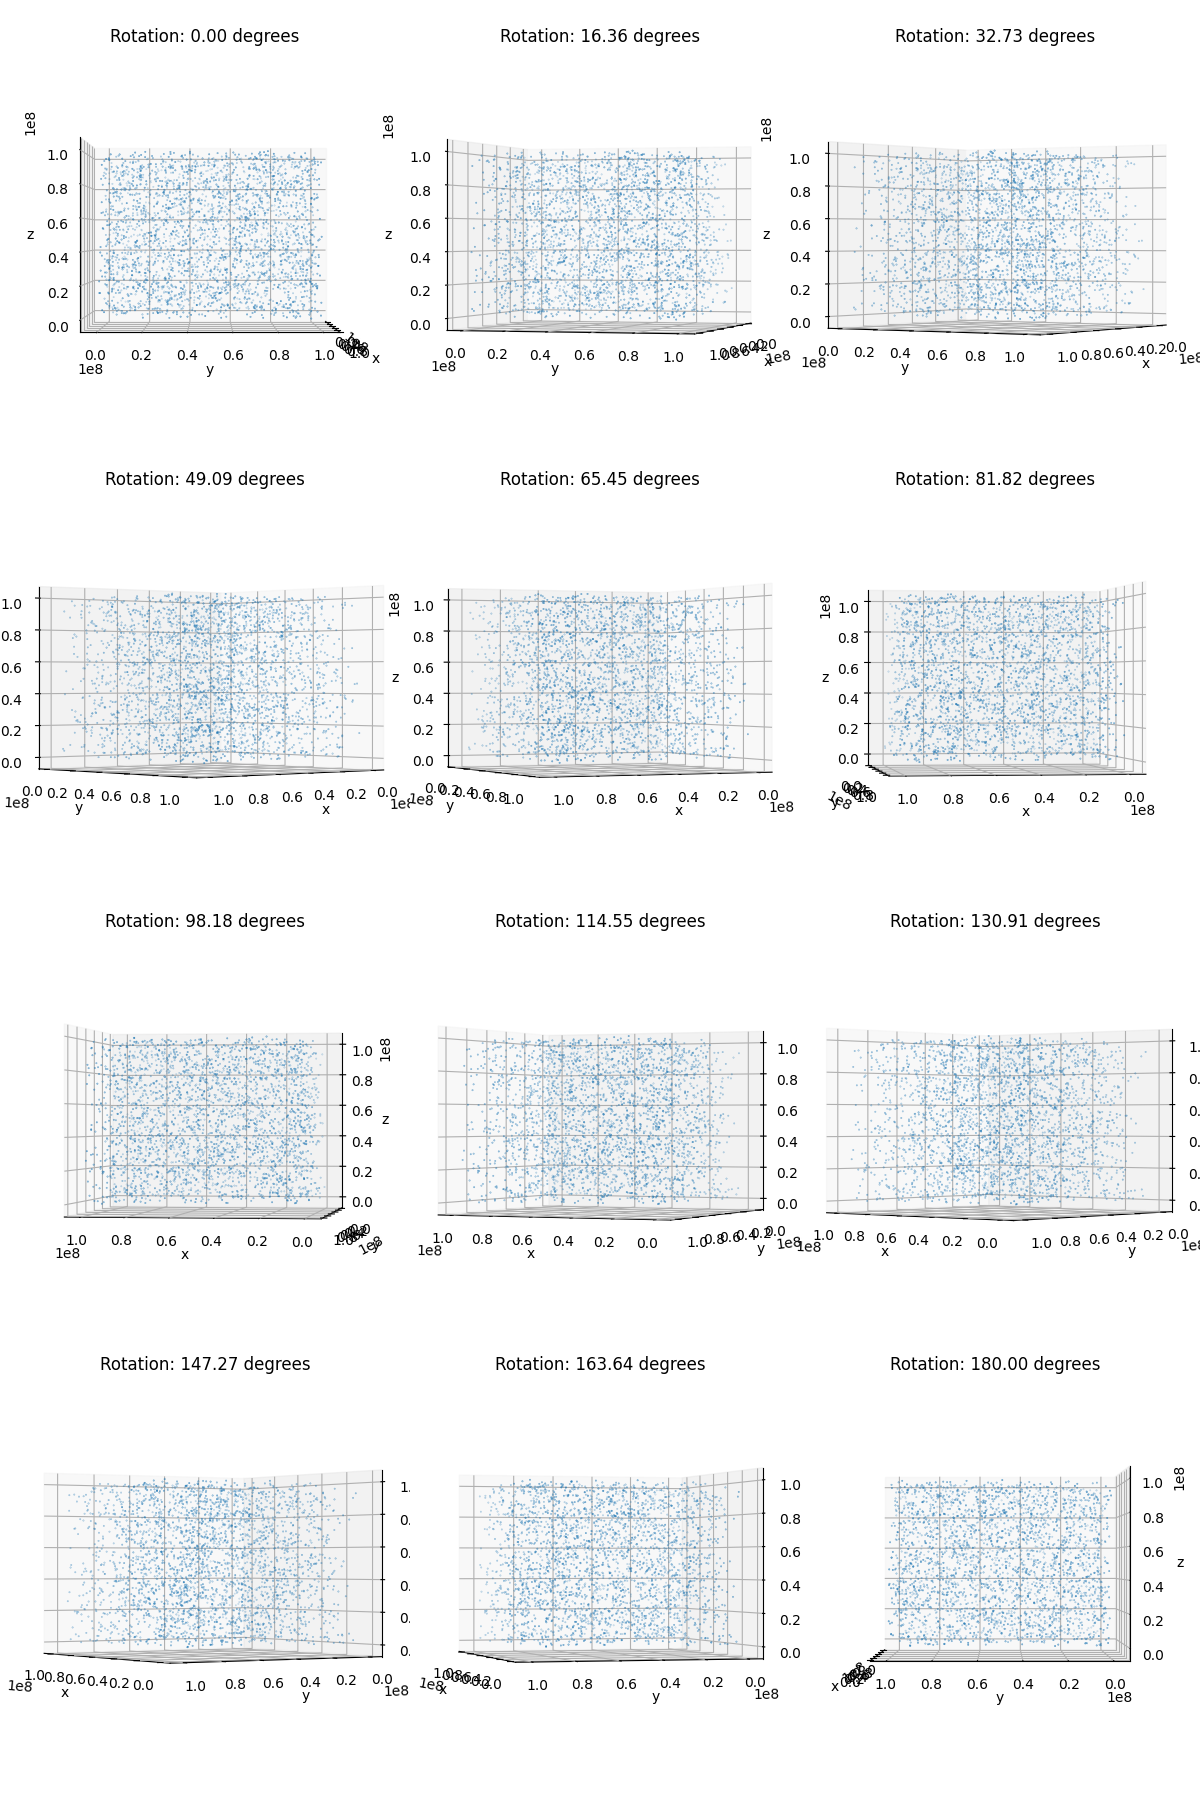
\includegraphics[width=\linewidth]{Results/q1b.png}
\end{figure}

\newpage
\section{Problem 2}
We are now asked to write a rejection method to generate exponential
deviates from another distribution. We first compare the Lorentians, Gaussians and power law to chose a distribution to draw samples from.

\begin{figure}[h!]
	\centering
	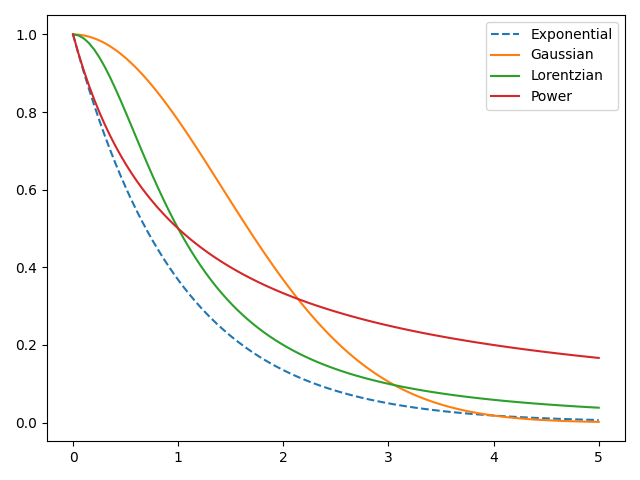
\includegraphics[width=0.5\linewidth]{Results/q2a.png}
\end{figure}

We first note that taking the gaussian distribution is not efficient since computing the value of a gaussian is more expensive than computing the value of an exponential function. Moreover, the gaussian decays faster than the exponential for large x and thus it does not bound it from above there.

Now we shift the power law by 1 so that it equals 1 at the origin. We notice that for $\alpha > 1$ in $(x + 1)^{-\alpha}$, the power law does not bound the exponential from above around 0, and hence we chose the lorentzian since it nicely bounds the exponential from above.
\begin{figure}[h!]
	\centering
	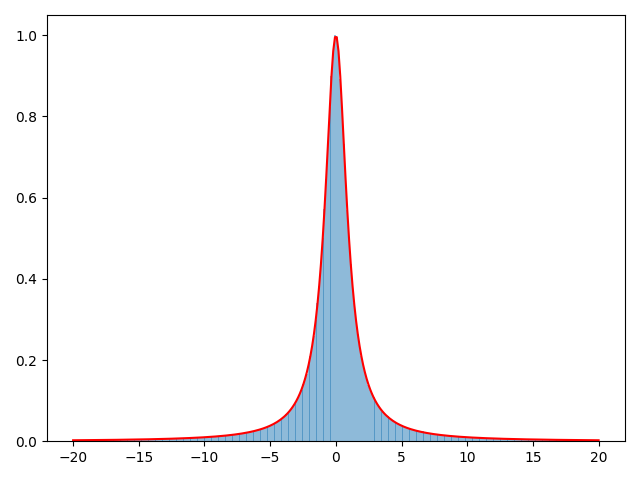
\includegraphics[width=0.45\linewidth]{Results/q2b.png}
	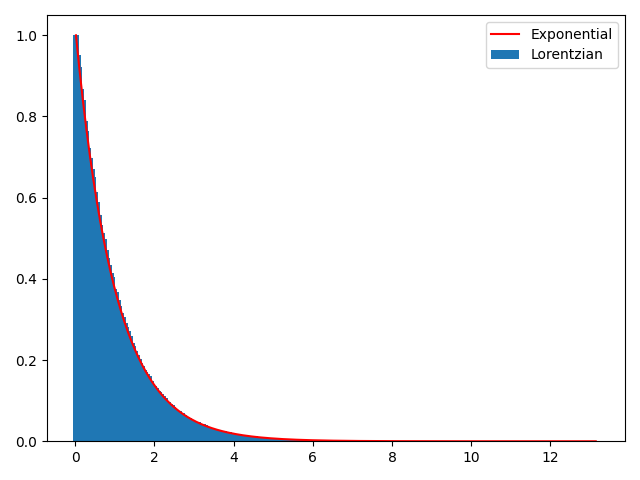
\includegraphics[width=0.45\linewidth]{Results/q2c.png}
\end{figure}

We note that our mapping nicely matches the lorentzian distribution, and our deviates also match the exponential curve.

We obtain an acceptance rate of about 64\%, and we could make it more efficient by finding a parent distribution with a tighter upper bound than the lorentzian we have.

\newpage
\section{Problem 3}
We repeat the above procedure, but now with a ratio of uniforms generator. Letting v be bounded by [0,1], we obtain an acceptance rate of about 50\%.

Since the acceptance is defined by
\begin{equation}
	0<u<e^{-v/2u}
\end{equation}
We can rearrange this so that
\begin{equation}
	0<v< -u ln(u^2)
\end{equation}
which has a maximum at
$$v = 2/e$$

By scaling our random v values to be bounded by [0, 2/e], we achieve an acceptance rate of about 67.9 \% while maintaining the exponential curve. While simpler, outperforms the lorentzian generator!

\begin{figure}[h!]
	\centering
	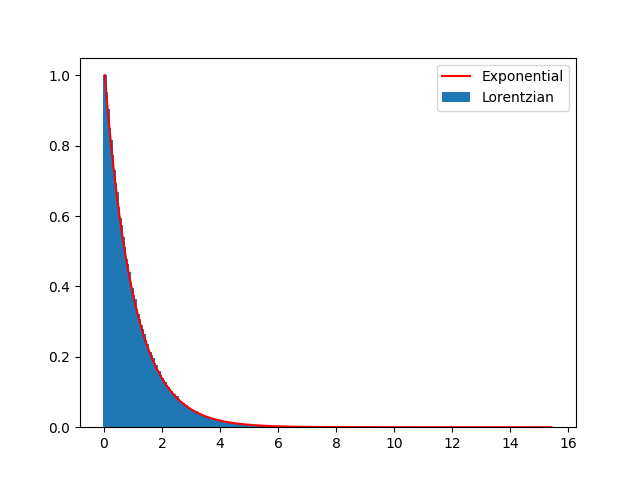
\includegraphics[width=0.45\linewidth]{Results/q3.png}
\end{figure}

\end{document}
